\documentclass[a4paper,12pt]{article}
\usepackage{amsmath, amssymb, graphicx}
\usepackage[margin=1in]{geometry}
\setlength\parindent{0pt}

\begin{document}

\title{Nested Bending}
\author{}
\date{}
\maketitle

\section*{Introduction}
In the code attached, we observe the bending of nested geodesics of a unit circle at an angle given as input for each geodesic.
The geodesics are also input by the user. There are however, certain constraints in the input parameters:
\begin{itemize}
    \item n(number of geodesics) $\in \mathbb{N}$.
    \item The points specifying the geodesic are entered as angular coordinates. Angles $\in (-2\pi, 2\pi)$.
    \item None of the geodesics should intersect each other; however, they are allowed to be nested.
    \item The angles of bending are required to be in the range (-$\pi$, $\pi$].
\end{itemize}

\section*{Logic}

\subsection*{1. Input Parameters}
The code takes the following inputs:
\begin{itemize}
    \item \( n \): The number of pairs.
    \item \( \text{angles} = \{(\theta_1, \theta_2)_i \}_{i=1}^n \): A list of angle pairs for each segment, where \( \theta_1 \) and \( \theta_2 \) are the start and end angles of the segment.
    \item \( \text{bendingAngles} = \{ \beta_i \}_{i=1}^n \): A list of bending angles corresponding to each pair.
\end{itemize}

The input procedure is:
\begin{itemize}
    \item The user is prompted to enter the number of pairs \( n \).
    \item The user is then asked to enter the angle pairs and bending angles for each pair.
    \item The above step is done n times.
\end{itemize}

Sample input:

{\centering
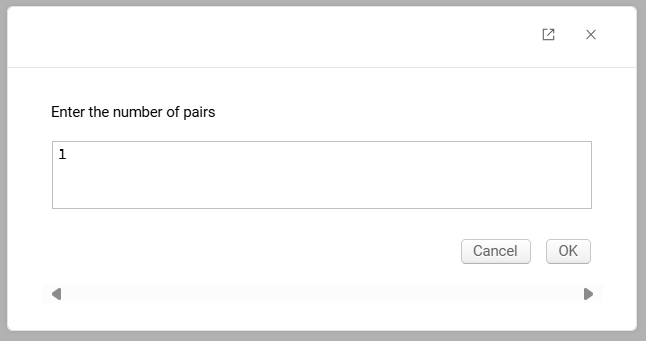
\includegraphics[width = 0.5\textwidth]{Entering Number of Pairs.png}\\
Entering number of pairs\\
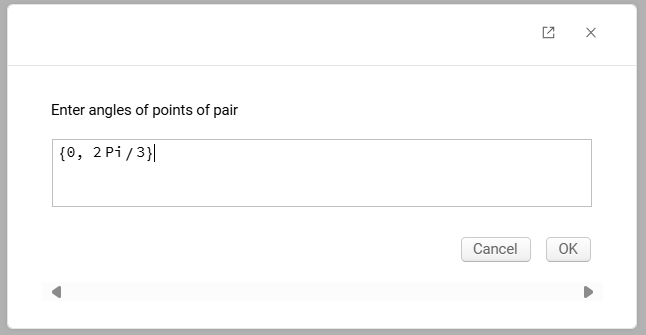
\includegraphics[width = 0.5\textwidth]{Entering the pair of points.png}\\
Entering the pair of points\\
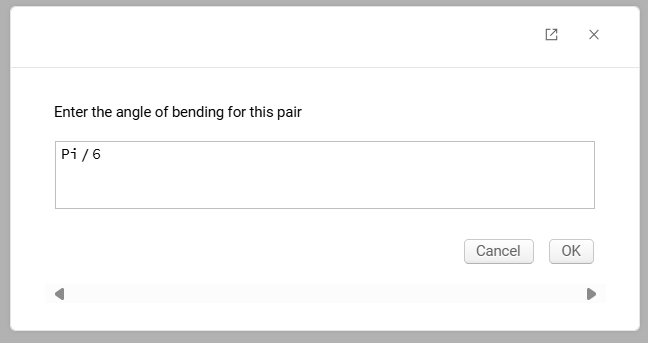
\includegraphics[width = 0.5\textwidth]{Entering the bending angle.png}\\
Entering the bending angle\\
}\par



\subsection*{2. Transformation Procedure}
For each pair \( i \):
\begin{enumerate}
    \item The points on the unit circle corresponding to the angles are calculated as:
    \[
    P_1 = (\cos(\theta_1), \sin(\theta_1)), \quad P_2 = (\cos(\theta_2), \sin(\theta_2)).
    \]

    \item The geodesic, if first mapped to the right hemisphere, which is then mapped to the positive real axis using two Mobius transformations.
    Then, the $\mathbb{R}^+$ axis is bent by the angle $\beta_i$. Then, finally the bent line is mapped back using the inverse of the previous Mobius transformations.
    The inverse Mobius transformations are given by:


    $$\mathbb{R}^+ \to Right\;Hemisphere: \frac{x+2i}{-ix+2}$$
    $$Right\;Hemisphere \to Geodesic: \frac{a_ix+b_i}{c_ix+d_i}$$
    $$k = \|P_1 + P_2\|, $$
    $$\text{const} = \frac{-\frac{2-k}{k}(P_1 + P_2) + i(P_2 - P_1)}{\frac{2-k}{k}(P_1 + P_2) + i(P_2 - P_1)},$$
    $$c_i = \sqrt{\frac{1}{\text{const}(\frac{(P_1 + P_2)}{2} - i \cdot \text{const} \cdot \frac{(P_1 - P_2)}{2}) - (\frac{(P_1+P_2)(2-k)}{(2k)}-const\cdot\frac{(P_1+P_2)}{k}-i\cdot const\cdot\frac{P_1-P_2}{2})}}.$$
    $$d_i = c_i\cdot const$$
    $$a_i = c_i\cdot \frac{P_1+P_2}{2}-i\cdot d_i\cdot \frac{P_2-P_1}{2}$$
    $$b_i = c_i\cdot \frac{(P_1+P_2)(2-k)}{2k}+d_i\cdot\left( \frac{P_1+P_2}{k} + i\cdot\frac{P_2-P_1}{2}\right)$$
    
\end{enumerate}
Thus, the geodesic is transformed by applying the above transformations to the bent $\mathbb{R}^+$ axis in the same order.

\subsection*{3. Tree Formation}
In the case of nested geodesics, we relate the bigger one as the parent of the ones that are immediately inside it. Therefore, we have a forest
of trees where the biggest geodesic in each connected component is the root of the tree. The visualization is done recursively by drawing the parent first and then the children.\\

Now, in order to apply the transformations, we first transform the parent and then apply the transformations to the children. This is done by composing the parent's transformation with the child's transformation. The transformation of the child is applied first. The transformation of the parent is then applied to the transformed geodesic. This is done recursively for all the children of the parent.

\subsection*{4. Output Visualization}
The graphical output consists of:
\begin{itemize}
    \item The unit circle.
    \item Parametric plots of the transformed segments.
    \item Recursive visualizations of parent-child relationships.
\end{itemize}

The final visualization is rendered using the \texttt{Show[]} function to combine all graphical elements.

\section*{Test Cases}
For each test case, the following inputs are used:
\begin{itemize}
    \item \( n \): Number of pairs.
    \item \( \text{angles} \): List of angle pairs.
    \item \( \text{bendingAngles} \): List of bending angles.
\end{itemize}

The resulting visualization is shown below:

\subsection*{Test Case 1}
\textbf{Inputs:}
\begin{itemize}
    \item \( n = 2 \)
    \item \( \text{angles} = \{(0, 2\pi/3), (\pi/6, \pi/2)\} \)
    \item \( \text{bendingAngles} = \{\pi/4, -\pi/6\} \)
\end{itemize}
\textbf{Output:}\\

{\centering
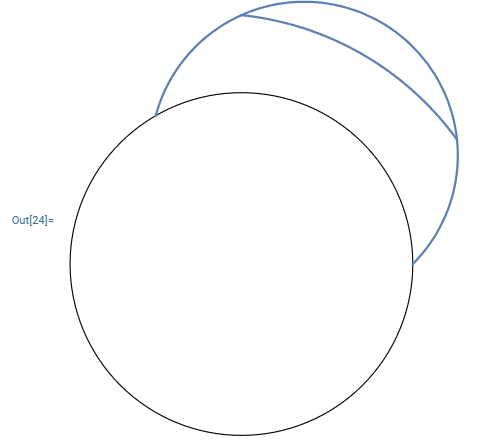
\includegraphics[height = 0.4\textheight]{Test 1.png}\\
}\par

Note here that, ${0, 2\pi/3}$ marks the parent of the tree and ${\pi/6, \pi/2}$ marks the child. The parent is bent by $\pi/4$ and the child is bent by $-\pi/6$.
Thus, in the figure, the outermost arc, represents the bending of ${0, 2\pi/3}$ and the inner arc represents the bending of ${\pi/6, \pi/2}$. Thus, the net result would
be the inner arc being bent by $-\pi/6$ with respect to the outer arc.

%\includegraphics[width=0.8\textwidth]{test_case_1.png}

\subsection*{Test Case 2}
\textbf{Inputs:}
\begin{itemize}
    \item \( n = 3 \)
    \item \( \text{angles} = \{(0, \pi/3), (\pi/6, \pi/4), (\pi/2, 2\pi/3)\} \)
    \item \( \text{bendingAngles} = \{\pi/6, -\pi/4, \pi/3\} \)

\end{itemize}
\textbf{Output:}\\

{\centering
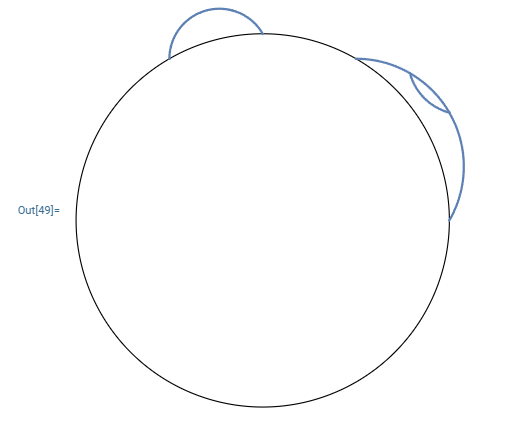
\includegraphics[height = 0.4\textheight]{Test 2.png}\\
}\par

\subsection*{Test Case 3}
\textbf{Inputs:}
\begin{itemize}
    \item \( n = 4 \)
    \item \( \text{angles} = \{(0, 2\pi/3), (\pi/6, \pi/2), (\pi/4, \pi/3), (5\pi/6, \pi)\} \)
    \item \( \text{bendingAngles} = \{\pi/6, \pi/4, \pi/3, \pi/6\} \)
\end{itemize}
\textbf{Output:}\\

{\centering
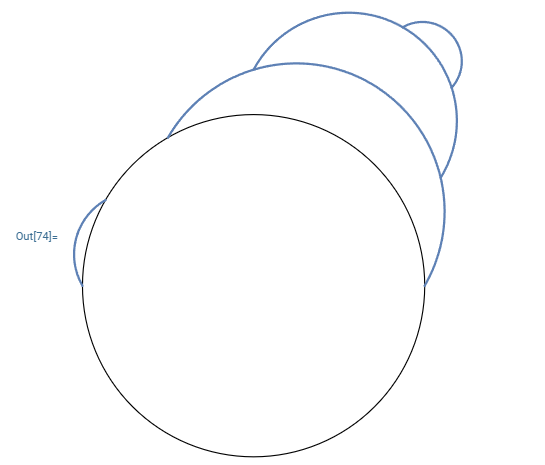
\includegraphics[height = 0.37\textheight]{Test 3.png}\\
}\par

\end{document}
